\documentclass{article}

% Margins and spacing
\usepackage[a4paper, margin=.7in]{geometry}
% Math packages
\usepackage{amsmath}
\usepackage{amssymb}
% Placement of figures, tables, algorithms, etc.
\usepackage{float}
% Algorithms
\usepackage{algorithm}
\usepackage{algpseudocode}
\usepackage{tikz}

% No section numbering
\setcounter{secnumdepth}{0}
% No paragraph indentation
\setlength{\parindent}{0pt}

% Define custom commands
%% Operators
\DeclareMathOperator*{\argmin}{arg\,min}
\DeclareMathOperator*{\argmax}{arg\,max}
%% Manually indented state in algorithmic environment
\newcommand{\IndentState}{\State \hspace{1em}}

\title{CSCI-570 Homework 5 Solutions}
\author{
  Naman Chhibbar \\
  USC ID: 7709-8548-02
}
\date{}

% Document body
\begin{document}
\maketitle

\section{Problem 1}
  \begin{itemize}
    \item[(a)] Consider the following flow network with $s$ as the source and $t$ as the sink with the capacities given on the edges: \\
    \begin{center}
      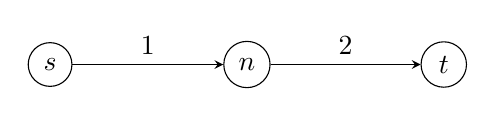
\begin{tikzpicture}[node distance=2.5cm, auto, >=stealth, node style/.style={circle, draw}]
        \node (s) [node style] {$s$};
        \node (n) [node style, right of=s] {$n$};
        \node (t) [node style, right of=n] {$t$};
        \draw[->] (s) -- node {1} (n);
        \draw[->] (n) -- node {2} (t);
      \end{tikzpicture}
    \end{center}
    It is easy to see that the maximum flow is 1, which is less than the capacity of the edge $(n, t)$ but more than 0, hence disproving the statement.

    \item[(b)] Consider the same flow network as in part (a).
    We can see that there is only one possible max flow mentioned in part (a) (there is only one path from $s$ to $t$).
    Since there are no other max flows and we have the same issue on the edge $(n, t)$, this statement is also false.

    \item[(c)] Consider the following flow network with $s$ as the source and $t$ as the sink with all edges having distinct capacities:
    \begin{center}
      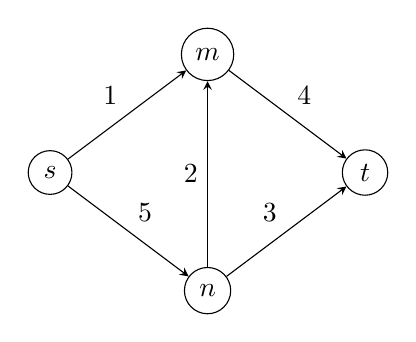
\begin{tikzpicture}[node distance=2.5cm, auto, >=stealth, node style/.style={circle, draw}]
        \node[node style] (m) at (0, 1.5) {$m$};
        \node[node style] (s) at (-2, 0) {$s$};
        \node[node style] (t) at (2, 0) {$t$};
        \node[node style] (n) at (0, -1.5) {$n$};
        \draw[->] (s) -- node {1} (m);
        \draw[->] (s) -- node {5} (n);
        \draw[->] (n) -- node{2} (m);
        \draw[->] (m) -- node {4} (t);
        \draw[->] (n) -- node {3} (t);
      \end{tikzpicture}
    \end{center}
    The maximum flow in this network is 6 shown as follows:
    \begin{center}
      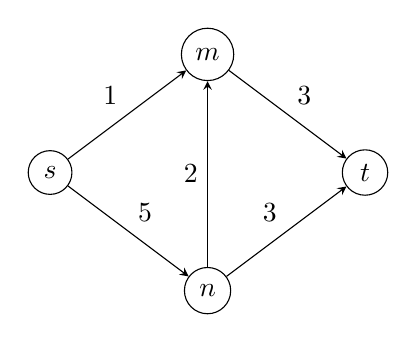
\begin{tikzpicture}[node distance=2.5cm, auto, >=stealth, node style/.style={circle, draw}]
        \node[node style] (m) at (0, 1.5) {$m$};
        \node[node style] (s) at (-2, 0) {$s$};
        \node[node style] (t) at (2, 0) {$t$};
        \node[node style] (n) at (0, -1.5) {$n$};
        \draw[->] (s) -- node {1} (m);
        \draw[->] (s) -- node {5} (n);
        \draw[->] (n) -- node{2} (m);
        \draw[->] (m) -- node {3} (t);
        \draw[->] (n) -- node {3} (t);
      \end{tikzpicture}
    \end{center}
    Also, we have two min cuts here: $(\{s\}, \{m, n, t\})$ and $(\{s, n\}, \{m, t\})$.
    Hence, this statement is false as well.

    \item[(d)] Consider the same flow network as in part (c), but with $\delta = 1$ added to all the capacities:
    \begin{center}
      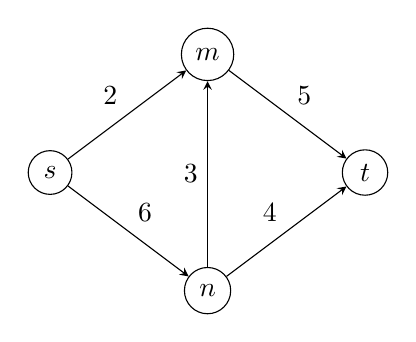
\begin{tikzpicture}[node distance=2.5cm, auto, >=stealth, node style/.style={circle, draw}]
        \node[node style] (m) at (0, 1.5) {$m$};
        \node[node style] (s) at (-2, 0) {$s$};
        \node[node style] (t) at (2, 0) {$t$};
        \node[node style] (n) at (0, -1.5) {$n$};
        \draw[->] (s) -- node {2} (m);
        \draw[->] (s) -- node {6} (n);
        \draw[->] (n) -- node{3} (m);
        \draw[->] (m) -- node {5} (t);
        \draw[->] (n) -- node {4} (t);
      \end{tikzpicture}
    \end{center}
    The maximum flow in this network is 8:
    \begin{center}
      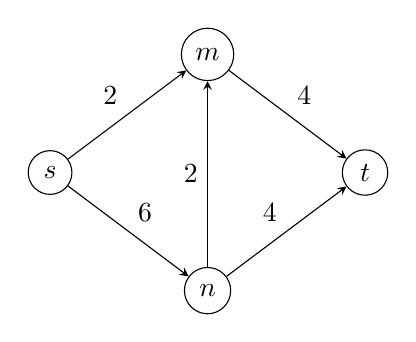
\begin{tikzpicture}[node distance=2.5cm, auto, >=stealth, node style/.style={circle, draw}]
        \node[node style] (m) at (0, 1.5) {$m$};
        \node[node style] (s) at (-2, 0) {$s$};
        \node[node style] (t) at (2, 0) {$t$};
        \node[node style] (n) at (0, -1.5) {$n$};
        \draw[->] (s) -- node {2} (m);
        \draw[->] (s) -- node {6} (n);
        \draw[->] (n) -- node{2} (m);
        \draw[->] (m) -- node {4} (t);
        \draw[->] (n) -- node {4} (t);
      \end{tikzpicture}
    \end{center}
    But, notice the fact that the min cut $(\{s, n\}, \{m, t\})$ in the original network is no longer a min cut in this new network (it has a capacity of 9).
    Hence, this statement is false too.

    \item[(e)] This statement is true.
    This is because on multiplying all capacities by a constant, the capacities of all cuts (not just min cuts) also get multiplied by the same constant. \\
    Proof: Consider any cut $(S, T)$ and let the capacities of the edges going from $S$ to $T$ be $c_1, c_2, \ldots, c_k$.
    Let the constant be $\delta$.
    The capacity of this cut before multiplying by $\delta$ is:
    \[ C = \sum_{i=1}^{k} c_i \]
    After multiplying all capacities by $\delta$, the new capacity of this cut is:
    \[ C' = \sum_{i=1}^{k} \delta c_i = \delta \sum_{i=1}^{k} c_i = \delta C \]
    Therefore, since the capacities of all cuts are also multiplied, the min cuts will remain the same.
  \end{itemize}

\section{Problem 2}
  \begin{itemize}
    \item[(a)] Here is the required example:
    \begin{center}
      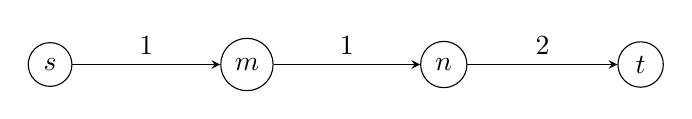
\begin{tikzpicture}[node distance=2.5cm, auto, >=stealth]
        \node (s) [circle, draw] {$s$};
        \node (m) [circle, draw, right of=s] {$m$};
        \node (n) [circle, draw, right of=m] {$n$};
        \node (t) [circle, draw, right of=n] {$t$};
        \draw[->] (s) -- node {1} (m);
        \draw[->] (m) -- node {1} (n);
        \draw[->] (n) -- node {2} (t);
      \end{tikzpicture}
    \end{center}
    Since there is a single path from $s$ to $t$, we have a unique max flow.
    But, we have two min cuts here: $(\{s\}, \{m, n, t\})$ and $(\{s, m\}, \{n, t\})$.

    \item[(b)] The network used in problem 1 part (d) works here:
    \begin{center}
      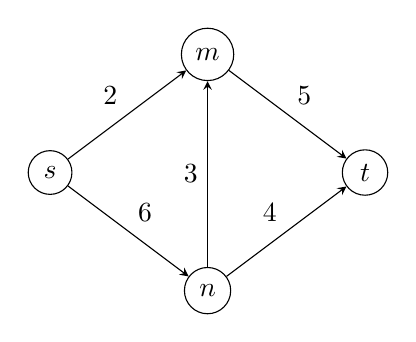
\begin{tikzpicture}[node distance=2.5cm, auto, >=stealth, node style/.style={circle, draw}]
        \node[node style] (m) at (0, 1.5) {$m$};
        \node[node style] (s) at (-2, 0) {$s$};
        \node[node style] (t) at (2, 0) {$t$};
        \node[node style] (n) at (0, -1.5) {$n$};
        \draw[->] (s) -- node {2} (m);
        \draw[->] (s) -- node {6} (n);
        \draw[->] (n) -- node{3} (m);
        \draw[->] (m) -- node {5} (t);
        \draw[->] (n) -- node {4} (t);
      \end{tikzpicture}
    \end{center}
    We have two max flows here of capacity 8:
    \begin{center}
      \begin{tikzpicture}
        \matrix[column sep=2cm]{
          \node (G1) {
            \begin{tikzpicture}[node distance=2.5cm, auto, >=stealth, node style/.style={circle, draw}]
              \node[node style] (m) at (0, 1.5) {$m$};
              \node[node style] (s) at (-2, 0) {$s$};
              \node[node style] (t) at (2, 0) {$t$};
              \node[node style] (n) at (0, -1.5) {$n$};
              \draw[->] (s) -- node {2} (m);
              \draw[->] (s) -- node {6} (n);
              \draw[->] (n) -- node{3} (m);
              \draw[->] (m) -- node {5} (t);
              \draw[->] (n) -- node {3} (t);
            \end{tikzpicture}
          }; &
          \node (G2) {
            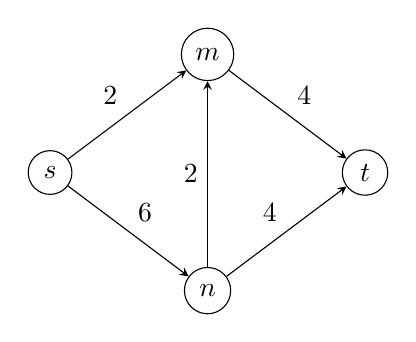
\begin{tikzpicture}[node distance=2.5cm, auto, >=stealth, node style/.style={circle, draw}]
              \node[node style] (m) at (0, 1.5) {$m$};
              \node[node style] (s) at (-2, 0) {$s$};
              \node[node style] (t) at (2, 0) {$t$};
              \node[node style] (n) at (0, -1.5) {$n$};
              \draw[->] (s) -- node {2} (m);
              \draw[->] (s) -- node {6} (n);
              \draw[->] (n) -- node{2} (m);
              \draw[->] (m) -- node {4} (t);
              \draw[->] (n) -- node {4} (t);
            \end{tikzpicture}
          }; \\
        };
      \end{tikzpicture}
    \end{center}
    But, we have a unique min cut: $(\{s\}, \{m, n, t\})$.

    \item[(c)] Plan:
    \begin{itemize}
      \item Calculate the max flow $f$ and the residual graph $G_f$ using Ford-Fulkerson algorithm.
      \item Get the set of vertices $S$ reachable from the source $s$ in $G_f$ using BFS.
      \item Invert all the edges in $G_f$.
      \item Get the set of vertices $T$ from which we can reach the sink $t$ in the inverted $G_f$ using BFS.
      \item If $|S| + |T| = |V|$, then the min cut is unique.
    \end{itemize}
    Intuition: If there exists a set of vertices $A$ not reachable from $s$ and we can not reach $t$ from it in $G_f$, we can add $A$ to $S$ or $T$ to get another min cut since the edges going from $S$ to $A$ and from $A$ to $T$ are saturated (otherwise, we could reach $A$ from $s$ or reach $t$ from $A$ in $G_f$). \\
    Assuming we have the \texttt{FordFulkerson} and \texttt{BFS} functions implemented, here is the complete algorithm:
    \begin{algorithm}
      \caption{Unique Min Cut}
      \begin{algorithmic}[1]
        \Function{Unique-Min-Cut}{$G, s, t$}
          \State $f, G_f \gets$ \Call{FordFulkerson}{$G, s, t$}
          \State $S \gets$ \Call{BFS}{$G_f, s$}
          \State Initialize empty edge set $E'$
          \For{each $(u, v) \in E(G_f)$} \Comment{$E(G_f)$ is the set of edges in $G_f$}
            \State Add edge $(v, u)$ to $E'$
          \EndFor
          \State Initialize graph $G' = (V(G_f), E')$ \Comment{$V(G_f)$ is the set of vertices in $G_f$}
          \State $T \gets$ \Call{BFS}{$G', t$}
          \State \Return $|S| + |T| = |V|$ \Comment{Here = is a comparator, not assignment}
        \EndFunction
      \end{algorithmic}
    \end{algorithm} \\
    Since we know that Ford-Fulkerson algorithm, BFS, and inverting the edges all run in polynomial time, this algorithm runs in polynomial time as well (since the maximum number of edges in $G_f$ is $2|E|$, where $E$ is the set of edges in the original graph $G$).
  \end{itemize}

\section{Problem 3}
  \begin{itemize}
    \item[(a)] Plan:
    \begin{itemize}
      \item Compute the residual graph $G_f$ using $f$ of the updated graph $G'$.
      \item Run BFS from the source $s$ in $G_f$ to check if the sink $t$ is reachable.
      If yes, return the set of edges from $s$ to $t$ found by BFS.
      If not, return the same flow.
      \item Traverse the path found by BFS. If the current edge is a forward edge, increase the flow by 1 unit.
      Otherwise, decrease the flow by 1 unit (of the reverse edge in $G'$ since the backward edge is not actually present).
    \end{itemize}
    We will keep a flag with each edge in $G_f$ to indicate whether it is a forward edge or a backward edge.
    We assume that we have a \texttt{BFS} function implemented that returns the path from the input vertices.
    If no path exists, it returns an empty set.
    Here is the complete algorithm:
    \begin{algorithm}[H]
      \caption{Update Flow}
      \begin{algorithmic}[1]
        \Function{Update-Flow}{$G', f, s, t$}
          \State Initialize empty edge set $E_f$
          \For{each $(u, v) \in G'$}
            \If{$c(u, v) > f(u, v)$} \Comment{$c(u, v)$ is the capacity of edge $(u, v)$}
              \State Add $(u, v)$ to $E_f$ as a forward edge
            \EndIf
            \If{$f(u, v) > 0$}
              \State Add edge $(v, u)$ to $E_f$ as a backward edge
            \EndIf
          \EndFor
          \State Initialize graph $G_f = (V(G'), E_f)$ \Comment{$V(G')$ is the set of vertices in $G'$}
          \State $path \gets$ \Call{BFS}{$G_f, s, t$}
          \If{$path$ is empty}
            \State \Return $f$
          \EndIf
          \For{each $(u, v) \in path$}
            \If{$(u, v)$ is a forward edge}
              \State $f(u, v) \gets f(u, v) + 1$
            \Else
              \State $f(v, u) \gets f(v, u) - 1$
            \EndIf
          \EndFor
          \State \Return $f$
        \EndFunction
      \end{algorithmic}
    \end{algorithm}
    Since creating the residual graph $G_f$ takes $O(E)$ time and BFS takes $O(V + E)$ time, the overall time complexity of this algorithm is $O(V + E)$, where $V$ is the set of vertices and $E$ is the set of edges in $G'$.

    \item[(b)] Plan:
    \begin{itemize}
      \item Check if an edge is overflowing.
      \item If no edge is overflowing, return the same flow.
      \item If an edge $(u, v)$ is overflowing, find the paths of flow from the source $s$ to $u$ and from $v$ to the sink $t$ using BFS (this can be done by only searching the edges with positive flow from $s$ and $v$).
      \item Decrease the flow on all edges in these two paths by 1 unit.
      \item Compute the residual graph $G_f$ using the updated flow.
      \item Run BFS from the source $s$ in $G_f$ to check if the sink $t$ is reachable.
      If yes, return the set of edges from $s$ to $t$ found by BFS.
      If not, return the updated flow.
      \item Traverse the path found by BFS.
      If the current edge is a forward edge, increase the flow by 1 unit.
      Otherwise, decrease the flow by 1 unit of the reverse edge in $G'$ (since the backward edge is not actually present).
    \end{itemize}
    Once again, we will keep a flag with each edge in $G_f$ to indicate whether it is a forward edge or a backward edge.
    We assume that we have the original \texttt{BFS} function and the tweaked \texttt{BFS\_Flow} function (it can be easily done by adding an if statement) that only checks the edges with positive flow. \\
    Now, here is the complete algorithm:
    \begin{algorithm}[H]
      \caption{Fix Flow}
      \begin{algorithmic}[1]
        \Function{Fix-Flow}{$G', f, s, t$}
          \For{each $(u, v) \in G'$}
            \If{$f(u, v) > c(u, v)$} \Comment{$c(u, v)$ is the capacity of edge $(u, v)$}
              \State $path\_to\_u \gets$ \Call{BFS\_Flow}{$G', f, s, u$}
              \State $path\_from\_v \gets$ \Call{BFS\_Flow}{$G', f, v, t$}
              \For{each $(x, y) \in path\_to\_u \cup path\_from\_v$}
                \State $f(x, y) \gets f(x, y) - 1$
              \EndFor
              \State \textbf{break}
            \EndIf
          \EndFor
          \State Initialize empty edge set $E_f$
          \For{each $(u, v) \in G'$}
            \If{$c(u, v) > f(u, v)$} \Comment{$c(u, v)$ is the capacity of edge $(u, v)$}
              \State Add $(u, v)$ to $E_f$ as a forward edge
            \EndIf
            \If{$f(u, v) > 0$}
              \State Add edge $(v, u)$ to $E_f$ as a backward edge
            \EndIf
          \EndFor
          \State Initialize graph $G_f = (V(G'), E_f)$ \Comment{$V(G')$ is the set of vertices in $G'$}
          \State $path \gets$ \Call{BFS}{$G_f, s, t$}
          \If{$path$ is empty}
            \State \Return $f$
          \EndIf
          \For{each $(u, v) \in path$}
            \If{$(u, v)$ is a forward edge}
              \State $f(u, v) \gets f(u, v) + 1$
            \Else
              \State $f(v, u) \gets f(v, u) - 1$
            \EndIf
          \EndFor
          \State \Return $f$
        \EndFunction
      \end{algorithmic}
    \end{algorithm}
    Since creating the residual graph $G_f$ takes $O(E)$ time, BFS takes $O(V + E)$ time (even the modified one), and checking for an overflowing edge takes $O(E)$ time, the overall time complexity of this algorithm is $O(V + E)$, where $V$ is the set of vertices and $E$ is the set of edges in $G'$.
  \end{itemize}

\section{Problem 4}
  \begin{itemize}
    \item[(a)] This can be easily done by creating a flow network as follows:
    \begin{itemize}
      \item Create the vertex set $V' = V$ and add a source $s$ and a sink $t$ to $V'$.
      \item Create the edge set $E' = E$.
      Add edges from $s$ to each vertex in $X$ and from each vertex $S$ to $t$ to $E'$.
      \item Set the capacity of each edge to 1 (this ensures each path from every vertex in $X$ to every vertex in $S$ does not share an edge with some other path from $X$ to $S$).
      \item Run the Ford-Fulkerson algorithm on this flow network.
      \item Check if every vertex in $X$ has an outgoing flow of 1 and every vertex in $S$ has an incoming flow of 1 (this ensures we have a path from every vertex in $X$ to a vertex in $S$).
      If yes, return true, otherwise false.
    \end{itemize}
    Once again, we assume that we have the \texttt{FordFulkerson} function implemented.
    Here is the complete algorithm:
    \begin{algorithm}[H]
      \caption{Escape Problem}
      \begin{algorithmic}[1]
        \Function{Escape-Problem}{$G, X, S$}
          \State Initialize vertex set $V' = V(G)$ \Comment{$V(G)$ is the set of vertices in $G$}
          \State Add vertices $s$ and $t$ to $V'$
          \State Initialize edge set $E' = E(G)$ \Comment{$E(G)$ is the set of edges in $G$}
          \For{each $x \in X$}
            \State Add edge $(s, x)$ to $E'$
          \EndFor
          \For{each $s \in S$}
            \State Add edge $(s, t)$ to $E'$
          \EndFor
          \State Initialize graph $G' = (V', E')$
          \For{each $(u, v) \in E'$}
            \State Set capacity $c(u, v) = 1$
          \EndFor
          \State $f, G_f \gets$ \Call{FordFulkerson}{$G', s, t$}
          \For{each $(u, v) \in E'$}
            \If{$u \in X$ and $f(u, v) \neq 1$}
              \State \Return \textbf{False}
            \EndIf
            \If{$v \in S$ and $f(u, v) \neq 1$}
              \State \Return \textbf{False}
            \EndIf
          \EndFor
          \State \Return \textbf{True}
        \EndFunction
      \end{algorithmic}
    \end{algorithm}
    Since the Ford-Fulkerson algorithm runs in polynomial time and all of the loops are over edge sets, the overall time complexity of this algorithm is polynomial.
  \item[(b)] Here is our updated plan:
    \begin{itemize}
      \item Create the vertex set $V'$ by splitting each vertex $v$ into $v_{in}$ and $v_{out}$, and add a source $s$ and a sink $t$ to $V'$.
      \item Create the updated vertex sets $X' = \{x_{in} | x \in X\}$ and $S' = \{s_{out} | s \in S\}$.
      \item Create the edge set $E'$ by adding the edges $(u_{out}, v_{in})$ for each edge $(u, v) \in E$ and $(v_{in}, v_{out})$ for each vertex $v \in V$.
      Then, add edges from $s$ to each vertex in $X'$ and from each vertex in $S'$ to $t$ to $E'$.
      \item Set the capacity of each edge to 1 (this ensures each path from every vertex in $X$ to every vertex in $S$ does not share a vertex with some other path from $X$ to $S$).
      \item Run the Ford-Fulkerson algorithm on this flow network.
      \item Check if every vertex in $X'$ has an outgoing flow of 1 and every vertex in $S'$ has an incoming flow of 1 (this ensures we have a path from every vertex in $X'$ to a vertex in $S'$).
      If yes, return true, otherwise false.
    \end{itemize}
    Again, we assume that we have the \texttt{FordFulkerson} function implemented.
    Here is the complete algorithm:
    \begin{algorithm}[H]
      \caption{Enforced Escape Problem}
      \begin{algorithmic}[1]
        \Function{Enforced-Escape-Problem}{$G, X, S$}
          \State Initialize empty sets $V', E', X', S', Added\_Vertices, Added\_to\_X, Added\_to\_S$
          \For{each $(u, v) \in E$}
            \If{$u \notin Added\_Vertices$}
              \State Add vertices $u_{in}, u_{out}$ to $V'$
              \State Add edge $(u_{in}, u_{out})$ to $E'$
              \State Add $u$ to $Added\_Vertices$
            \EndIf
            \If{$v \notin Added\_Vertices$}
              \State Add vertices $v_{in}, v_{out}$ to $V'$
              \State Add edge $(v_{in}, v_{out})$ to $E'$
              \State Add $v$ to $Added\_Vertices$
            \EndIf
            \State Add edge $(u_{out}, v_{in})$ to $E'$
            \If{$u \in X$ and $u \notin Added\_to\_X$}
              \State Add $u_{in}$ to $X'$
              \State Add $u$ to $Added\_to\_X$
            \EndIf
            \If{$u \in S$ and $u \notin Added\_to\_S$}
              \State Add $u_{in}$ to $S'$
              \State Add $u$ to $Added\_to\_S$
            \EndIf
            \If{$v \in X$ and $v \notin Added\_to\_X$}
              \State Add $v_{out}$ to $X'$
              \State Add $v$ to $Added\_to\_X$
            \EndIf
            \If{$v \in S$ and $v \notin Added\_to\_S$}
              \State Add $v_{out}$ to $S'$
              \State Add $v$ to $Added\_to\_S$
            \EndIf
          \EndFor
          \State Initialize graph $G' = (V', E')$
          \For{each $(u, v) \in E'$}
            \State Set capacity $c(u, v) = 1$
          \EndFor
          \State $f, G_f \gets$ \Call{FordFulkerson}{$G', s, t$}
          \For{each $(u, v) \in E'$}
            \If{$u \in X'$ and $f(u, v) \neq 1$}
              \State \Return \textbf{False}
            \EndIf
            \If{$v \in S'$ and $f(u, v) \neq 1$}
              \State \Return \textbf{False}
            \EndIf
          \EndFor
          \State \Return \textbf{True}
        \EndFunction
      \end{algorithmic}
    \end{algorithm}
    Just as in part (a), since the Ford-Fulkerson algorithm runs in polynomial time and all of the loops are over edge sets, the overall time complexity of this algorithm is polynomial as well.
  \end{itemize}

\end{document}
